\documentclass[14pt]{extarticle}
\usepackage[english,ukrainian]{babel}
\usepackage[utf8]{inputenc}
\usepackage{amsmath,amssymb}
\usepackage{parskip}
\usepackage{graphicx}
\usepackage{xcolor}
\usepackage{tcolorbox}
\tcbuselibrary{skins}
\usepackage[framemethod=tikz]{mdframed}
\usepackage{chngcntr}
\usepackage{enumitem}
\usepackage{hyperref}
\usepackage{float}
\usepackage{subfig}
\usepackage{esint}
\usepackage[top=2.5cm, left=3cm, right=3cm, bottom=4.0cm]{geometry}
\usepackage[table]{xcolor}
\usepackage{algorithm}
\usepackage{algpseudocode}
\usepackage{listings}
\usepackage{xcolor}

\title{Контрольна робота \#1 з курсу ``Комплексний аналіз''}
\author{Студента 3 курсу групи МП-31 Захарова Дмитра}
\date{\today}

\begin{document}

\maketitle

\textbf{Варіант 5.}
\section*{Задача 1.} 

\textbf{Умова.} Знайти $\text{Re}\,(-i-1)^{1/3}$.

\textbf{Розв'язок.} Прочатку запишемо $-1-i$ в полярній формі. Помітимо, що:
\[
-1-i = -(1+i)=-\sqrt{2}e^{i\frac{\pi}{4} + 2\pi k i},\; k \in \mathbb{Z}
\]

Отже, якщо піднесемо до ступеня:
\[
(-1-i)^{1/3} = (-\sqrt{2}e^{i\pi / 4 + 2\pi k i})^{1/3} = -\sqrt[6]{2}e^{\frac{i\pi}{12} + \frac{2\pi k i}{3}},\; k\in\mathbb{Z}
\]

Тому дійсна частина:
\[
\text{Re} \, (-1-i)^{1/3} = -\sqrt[6]{2}\cos\left(\frac{\pi}{12}+\frac{2\pi k}{3}\right), \; k \in\mathbb{Z}
\]

\textit{Коментар.} По суті, ми розв'язували рівняння $z^3=-i-1$ і отримали 3 корні, якщо підставляти $k=0,1,2$.

\textbf{Відповідь.} $-\sqrt[6]{2}\cos\left(\frac{\pi}{12}+\frac{2\pi k}{3}\right), \; k \in\mathbb{Z}$

\pagebreak
\section*{Задача 2.} 

\textbf{Умова.} Знайти $\text{Im}\, (i\sqrt{3}-1)^{i-1}$.

\textbf{Розв'язок.} Використаємо той факт, що $z^w = e^{w \text{Log}\, z}$.

Тому переводимо $z=i\sqrt{3}-1$ у полярну форму:
\[
z = -1+i\sqrt{3} = 2\left(-\frac{1}{2}+i \frac{\sqrt{3}}{2}\right) = 2e^{\frac{2\pi i}{3}+2\pi k i}
\]

Тому:
\[
\text{Log}\, z = \text{Log}\, 2e^{\frac{2\pi i}{3} + 2\pi k i} = \log 2 + \frac{2\pi i}{3} + 2\pi k i
\]

Отже:
\[
\text{Im}\, (i\sqrt{3}-1)^{i-1} = \text{Im}\, e^{(i-1)(\log 2 + \frac{2\pi}{3} i + 2\pi k i)}
\]

Розкриємо дужки у ступені:
\begin{align*}
(i-1)\left(\log 2 + \frac{2\pi}{3} i + 2\pi k i\right) = i \log 2 - \frac{2\pi}{3} - 2\pi k - \log 2 - \frac{2\pi}{3} i - 2 \pi k i = \\
\left(-\frac{2\pi}{3} -\log 2 - 2\pi k\right) + i\left(\log 2 - \frac{2\pi}{3} - 2\pi k\right)
\end{align*}

Отже, уявна частна $e^{\text{цього виразу}}$:
\[
e^{-2\pi/3 - \log 2 - 2\pi k} \sin\left(\log 2 - \frac{2\pi}{3}\right)
\]

\textbf{Відповідь.} $e^{-2\pi/3 - \log 2 - 2\pi k} \sin\left(\log 2 - \frac{2\pi}{3}\right)$

\pagebreak
\section*{Задача 3.} 

\textbf{Умова.} Розв'язати рівняння $\sin z = -i$.

\textbf{Розв'язок.} Запишемо синус згідно комплексному означенню:
\[
\sin z \triangleq \frac{e^{iz}-e^{-iz}}{2i}
\]

Отже, якщо зробимо заміну $w=e^{iz}$:
\[
\frac{w-\frac{1}{w}}{2i} = -i \implies w-\frac{1}{w} = 2 \implies w^2 - 2w - 1 = 0 
\]

Розв'язуємо це квадрате рівняння:
\[
w = 1 \pm \sqrt{1 + 1} = 1 \pm \sqrt{2}
\]

Отже, або $e^{iz}=1+\sqrt{2}$, або $e^{iz}=1-\sqrt{2}$. 

В першому випадку $z = \frac{1}{i}(\log(1+\sqrt{2})+2\pi k i) = -i\log(1+\sqrt{2})+2\pi k$, у другому $z=-i\log(1-\sqrt{2})+2\pi k$.

Оскільки $1-\sqrt{2}<0$, то можна додатково розписати $\log(1-\sqrt{2})=\log(\sqrt{2}-1)+\pi i$ (використовуючи формулу $\log x = \log |x| + i \pi$ для $x<0$), тому другий коріень можна записати як $z=\pi+i \log(1+\sqrt{2}) + 2\pi k$

\textbf{Відповідь.} $z=-i\log(1 + \sqrt{2})+2\pi k, \; k \in \mathbb{Z}$ або $z=\pi +i \log(1+\sqrt{2})+2\pi k$.
\pagebreak
\section*{Задача 4.} 

\textbf{Умова.} Знайти точки, в яких функція $f(x+iy)=x^2+y^2-2x - 2ixy$ є диференційованою.

\textbf{Розв'язок.} Скористаємося умовою Коші-Рімана. В нашому випадку, якщо $f(x+iy)=u(x,y)+iv(x,y)$, то має виконуватись:
\[
u_x' = v_y' \wedge u_y' = -v_x'
\]

Маємо $u(x,y)=x^2+y^2-2x, v(x,y)=-2xy$. Тому:
\[
\begin{cases}
    2x-2 = -2x \\
    2y = 2y
\end{cases}
\]

Множина $(x,y)$, що є розв'язком цього рівняння, і є множиною точок, де функція є диференційованою. З першого рівняння $4x=2$, тобто $x=\frac{1}{2}$. З другого $y \in \mathbb{R}$. 

Отже, функція є диференційованою на прямій $x=\frac{1}{2}$.

\textbf{Відповідь.} На усіх точках на прямій $\text{Re} \, z = \frac{1}{2}$.

\pagebreak
\section*{Задача 5.}

\textbf{Умова.} Зобразити на площині ГМТ, які задовольняють умові $z=te^{-5\pi i/3},0 \leq t \leq 4$

\textbf{Розв'язок.} Знайдемо дійсні та уявні частини цього виразу:
\[
\text{Re} \, z = t \cos\left(-\frac{5\pi}{3}\right) = \frac{1}{2}t, \; \text{Im} \, z = t \sin\left(-\frac{5\pi}{3}\right) = \frac{\sqrt{3}}{2}t
\]

Отже, якщо розглянемо комплексну площину, то маємо параметризну криву:
\[
\{x,y\}(t) = \{t/2,\sqrt{3}t/2\}
\]

Це є прямою між $(0,0)$ та $(2,2\sqrt{3})$. Або, частина променю $\text{Arg}\, z = \pi/3$ між цими точками. Отже відповідь -- рис. \ref{fig:5}

\begin{figure}[H]
    \centering
    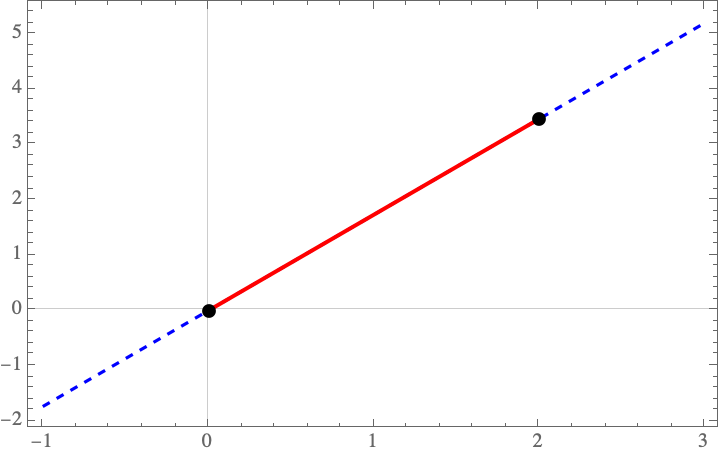
\includegraphics[width=0.7\textwidth]{images/test_1/plot_1.png}
    \caption{\textcolor{red}{Червоним} помічена відповідь, \textbf{чорним} точки $(0,0)$ та $(2,2\sqrt{3}$), \textcolor{blue}{синім} -- промінь}
    \label{fig:5}
\end{figure}
\vspace{5px}

\pagebreak
\section*{Задача 6.}

\textbf{Умова.} Зобразити ГМТ, які задовольняють умові
\[
\{z \in \mathbb{C}: |\text{Re}\, z + 1| < 1 \wedge |\text{Im}\, z - 1| > 1\}
\]

\textbf{Розв'язок.} Нехай $z = x + iy$. Тоді на $\mathbb{R}^2$ маємо наступне ГМТ:
\[
\{(x,y)\in\mathbb{R}^2:|x+1| < 1 \wedge |y-1| > 1\}
\]

Умова $|x+1|<1$ означає інтервал $(-2,0)$. 

Умова $|y-1|>1$ означає $\mathbb{R} \setminus [0,2] = (-\infty,0) \cup (2,+\infty)$.

Таким чином, наше ГМТ це декартовий добуток $(-2,0) \times (\mathbb{R} \setminus [0,2])$. Тому відповідь зображена на \ref{fig:6} (на пунктири на самому верху та низу не звертати увагу, область йде далі вгору і вниз).

\begin{figure}[H]
    \centering
    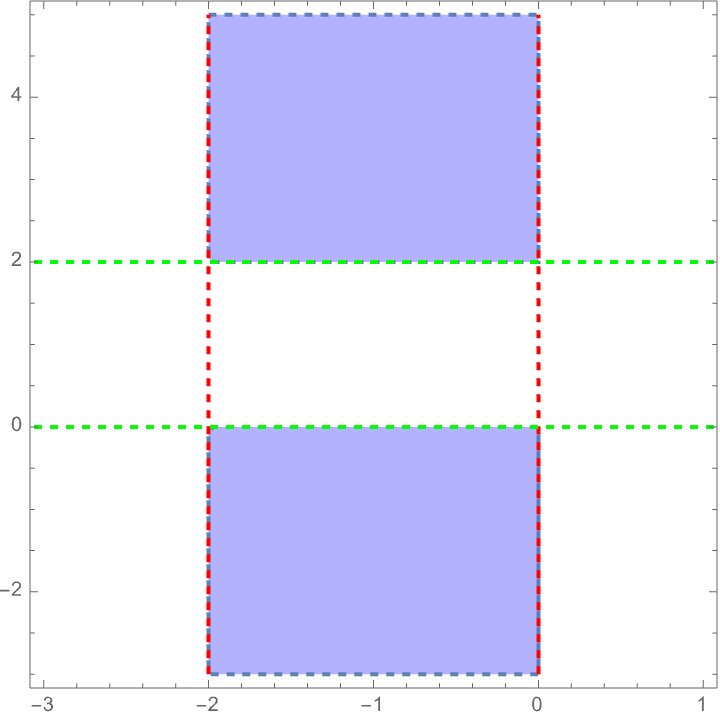
\includegraphics[width=0.6\textwidth]{images/test_1/plot_2.png}
    \caption{\textcolor{blue}{Синім} помічена відповідь. \textcolor{red}{червоним} -- прямі $x=-2,x=0$, \textcolor{green}{зеленим} -- прямі $y=0,y=2$}
    \label{fig:6}
\end{figure}
\vspace{5px}

\pagebreak
\section*{Задача 7.}

\textbf{Умова.} Відновити аналітичну функцію за її дійсною частиною: 
\[
u(x,y) = e^y \sin x + x^2 - y^2
\]

\textbf{Розв'язок.} Якщо функція аналітична, то мають виконуватись умови Коші-Рімана:
\[
u_x' = v_y' \wedge u_y'=-v_x'
\]

Отже, розв'яжемо це рівняння відносно $v(x,y)$. Маємо:
\[
\begin{cases}
    v_y' = e^y \cos x + 2x \\
    v_x' = -e^y\sin x + 2y
\end{cases}
\]

Якщо проінтегрувати перше рівняння, то отримаємо:
\[
v = \int \left(e^y \cos x + 2x\right)dy = e^y \cos x + 2xy + \varphi(x)
\]

Підставляємо у друге:
\[
-e^y \sin x + 2y + \varphi'(x) = -e^y \sin x + 2y \to \varphi'(x)=0 \to \varphi \equiv \text{const}
\]

Отже, остаточно:
\[
v(x,y) = e^y \cos x + 2xy + C, \; C = \text{const}
\]

\textbf{Відповідь.} $f(x+iy)=(e^y\sin x+x^2-y^2)+(e^y\cos x + 2x y + C)i, \; C = \text{const}$

\pagebreak
\section*{Задача 8.}

\textbf{Умова.} Спростити вираз $z=\frac{(2i+3)^2}{(2+i)(1-i)}$.

\textbf{Розв'язок.} Розпишемо чисельник та знаменник:
\[
(2i+3)^2 = (2i)^2 + 3^2 + 2 \cdot 2i \cdot 3 = 5 + 12i
\]
\[
(2+i)(1-i) = 2 - 2i + i - i^2 = 3-i
\]

Отже
\[
z = \frac{5+12i}{3-i} = \frac{(5+12i)(3+i)}{10} = \frac{15+5i+36i-12}{10} = \frac{3}{10} + \frac{41i}{10}
\]

\textbf{Відповідь.} $\frac{3}{10}+\frac{41}{10}i$

\end{document}

